\subsection{新增 PBE DFT Stage1+MatterSim Stage2：固定同一结构与模式}

本次直接读取已完成的PBE弛豫结构和DFPT模式，仅新增MatterSim Stage2，不重新弛豫结构或计算声子。三种材料各五个既定匹配通道，最强通道81点、其余四个通道各25点，共543个MatterSim构型。位移构造与原始QE PBE输入逐点核对，三个材料最大坐标差均小于$10^{-9}$\AA；Γ光学模选择、实际质量加权单位范数和动量守恒均通过核验。中心5$\times$5全部采用同一13列拟合。表~\ref{tab:cubic-all}与四阶表已加入PBE DFT+MS列，旧LDA基线没有被误标为PBE。

\begin{table}[!htbp]\centering\small
\caption{新增PBE DFT+MatterSim五通道误差。三四阶单位分别为$\cubunit$和$\quartunit$；全网格E为各材料181点的中心对齐能量MAE（meV/超胞），F为全部8766个原子力分量MAE（eV/\AA）。}\label{tab:pbe-dft-ms-metrics}
\allwidthtable{pbe_dft_ms_metrics}\end{table}

\begin{figure}[!htbp]\centering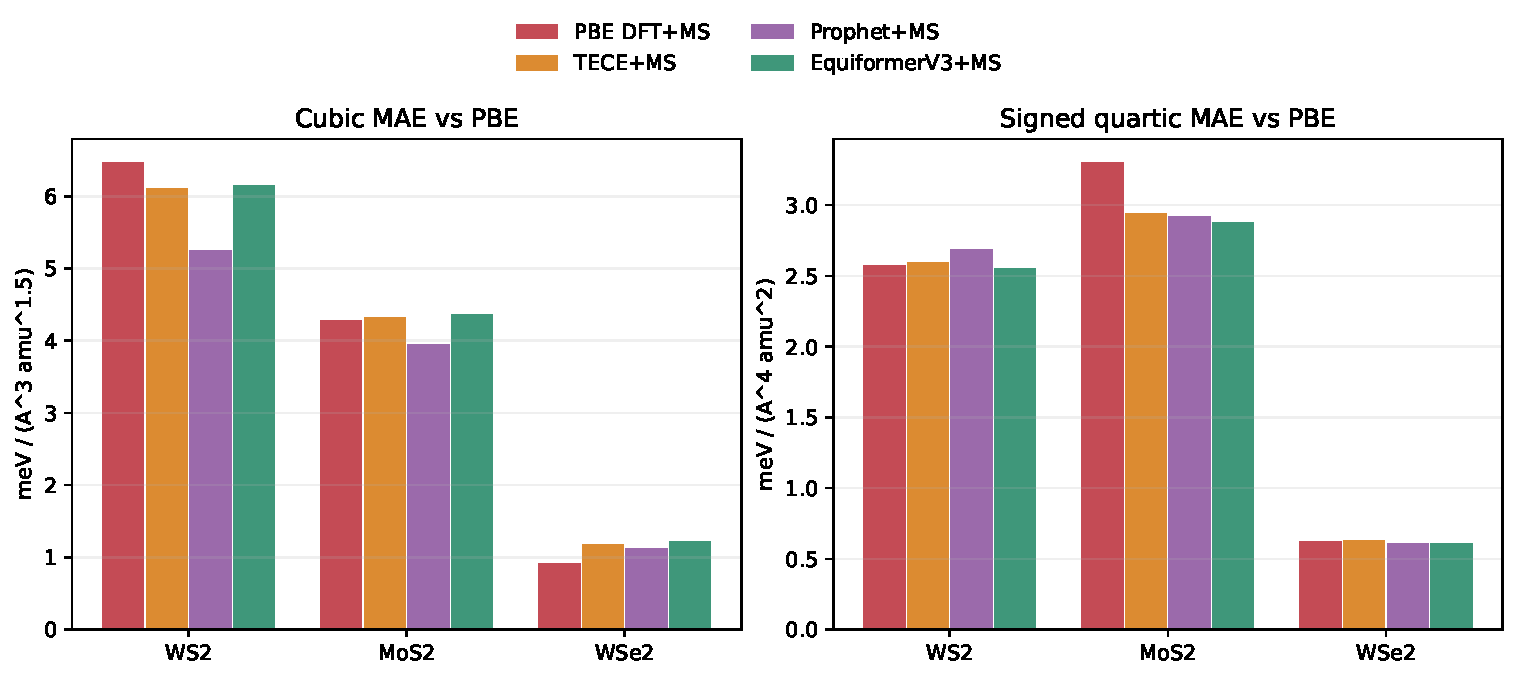
\includegraphics[width=0.94\textwidth]{figures/pbe_dft_ms_errors.pdf}
\caption{在同一新PBE参考下比较新DFT模式基线与三条全MLFF路线；全部比较最终物理通道的三阶强度和有符号四阶。}\label{fig:pbe-dft-ms-errors}\end{figure}

新PBE DFT+MatterSim的三阶MAE在WS$_2$/MoS$_2$/WSe$_2$为6.470/4.274/0.918，对照TECE+MatterSim的6.104/4.328/1.180：WSe$_2$改善较清楚，MoS$_2$差异较小，WS$_2$未改善。其四阶MAE为2.572/3.302/0.620，MoS$_2$反而高于TECE路线的2.939。这表明DFT模式基不能自动消除MatterSim势能面的高阶误差，也不能把原三条路线的偏差全部归因于Stage1。

\begin{table}[!htbp]\centering\small
\caption{新PBE DFT+MatterSim逐通道结果及中心5$\times$5误差。E为相对各自中心点的能量MAE（meV/超胞），F为原子力分量MAE（eV/\AA），拟合RMSE为模型势能与多项式之差（meV/超胞）；拟合残差不等于对DFT的误差。}\label{tab:pbe-dft-ms-details}
\allwidthtable{pbe_dft_ms_details}\end{table}

WS$_2$ $\Gamma8$--M6在完全相同PBE构型上再次得到QE $\PhiD=-1.4141$、MatterSim $+1.9304$ $\quartunit$，复现既有同构型诊断。MoS$_2$首通道的QE三阶强度94.809与新DFT+MS的89.630仍有差距，四阶则为7.557与14.226。模式与结构完全相同并未使这些差异消失，后续应针对Stage2势能形状和训练标签细节开展校准。

三条独立Slurm CPU作业每条分配8个线程，全部COMPLETED，每条调度墙钟57秒；包括一次加载的Stage2墙钟分别为46.49/46.59/45.88秒。它们是本次已选通道的小超胞性能，不代表完整6$\times$6候选扫描耗时。所有计算共占用3个节点，未超过全账号10节点限制。

公开接口已恢复DFT Stage1结果交接：\texttt{stage1 --model qe-dft}只导入已有DFPT数据，完整模式可接现有\texttt{stage2 screen/refine/audit}；已选详细通道通过\texttt{stage2 reference}直接计算同一QE网格。原DFT结构不经模型弛豫，且两类来源使用独立哈希身份和检查点。
\FloatBarrier
